\documentclass[twoside]{book}

% Packages required by doxygen
\usepackage{fixltx2e}
\usepackage{calc}
\usepackage{doxygen}
\usepackage[export]{adjustbox} % also loads graphicx
\usepackage{graphicx}
\usepackage[utf8]{inputenc}
\usepackage{makeidx}
\usepackage{multicol}
\usepackage{multirow}
\PassOptionsToPackage{warn}{textcomp}
\usepackage{textcomp}
\usepackage[nointegrals]{wasysym}
\usepackage[table]{xcolor}

% Font selection
\usepackage[T1]{fontenc}
\usepackage[scaled=.90]{helvet}
\usepackage{courier}
\usepackage{amssymb}
\usepackage{sectsty}
\renewcommand{\familydefault}{\sfdefault}
\allsectionsfont{%
  \fontseries{bc}\selectfont%
  \color{darkgray}%
}
\renewcommand{\DoxyLabelFont}{%
  \fontseries{bc}\selectfont%
  \color{darkgray}%
}
\newcommand{\+}{\discretionary{\mbox{\scriptsize$\hookleftarrow$}}{}{}}

% Page & text layout
\usepackage{geometry}
\geometry{%
  a4paper,%
  top=2.5cm,%
  bottom=2.5cm,%
  left=2.5cm,%
  right=2.5cm%
}
\tolerance=750
\hfuzz=15pt
\hbadness=750
\setlength{\emergencystretch}{15pt}
\setlength{\parindent}{0cm}
\setlength{\parskip}{3ex plus 2ex minus 2ex}
\makeatletter
\renewcommand{\paragraph}{%
  \@startsection{paragraph}{4}{0ex}{-1.0ex}{1.0ex}{%
    \normalfont\normalsize\bfseries\SS@parafont%
  }%
}
\renewcommand{\subparagraph}{%
  \@startsection{subparagraph}{5}{0ex}{-1.0ex}{1.0ex}{%
    \normalfont\normalsize\bfseries\SS@subparafont%
  }%
}
\makeatother

% Headers & footers
\usepackage{fancyhdr}
\pagestyle{fancyplain}
\fancyhead[LE]{\fancyplain{}{\bfseries\thepage}}
\fancyhead[CE]{\fancyplain{}{}}
\fancyhead[RE]{\fancyplain{}{\bfseries\leftmark}}
\fancyhead[LO]{\fancyplain{}{\bfseries\rightmark}}
\fancyhead[CO]{\fancyplain{}{}}
\fancyhead[RO]{\fancyplain{}{\bfseries\thepage}}
\fancyfoot[LE]{\fancyplain{}{}}
\fancyfoot[CE]{\fancyplain{}{}}
\fancyfoot[RE]{\fancyplain{}{\bfseries\scriptsize Generated by Doxygen }}
\fancyfoot[LO]{\fancyplain{}{\bfseries\scriptsize Generated by Doxygen }}
\fancyfoot[CO]{\fancyplain{}{}}
\fancyfoot[RO]{\fancyplain{}{}}
\renewcommand{\footrulewidth}{0.4pt}
\renewcommand{\chaptermark}[1]{%
  \markboth{#1}{}%
}
\renewcommand{\sectionmark}[1]{%
  \markright{\thesection\ #1}%
}

% Indices & bibliography
\usepackage{natbib}
\usepackage[titles]{tocloft}
\setcounter{tocdepth}{3}
\setcounter{secnumdepth}{5}
\makeindex

% Hyperlinks (required, but should be loaded last)
\usepackage{ifpdf}
\ifpdf
  \usepackage[pdftex,pagebackref=true]{hyperref}
\else
  \usepackage[ps2pdf,pagebackref=true]{hyperref}
\fi
\hypersetup{%
  colorlinks=true,%
  linkcolor=blue,%
  citecolor=blue,%
  unicode%
}

% Custom commands
\newcommand{\clearemptydoublepage}{%
  \newpage{\pagestyle{empty}\cleardoublepage}%
}

\usepackage{caption}
\captionsetup{labelsep=space,justification=centering,font={bf},singlelinecheck=off,skip=4pt,position=top}

%===== C O N T E N T S =====

\begin{document}

% Titlepage & ToC
\hypersetup{pageanchor=false,
             bookmarksnumbered=true,
             pdfencoding=unicode
            }
\pagenumbering{alph}
\begin{titlepage}
\vspace*{7cm}
\begin{center}%
{\Large \char`\"{}\+University Conference Center System\char`\"{} \\[1ex]\large 3.\+2 }\\
\vspace*{1cm}
{\large Generated by Doxygen 1.8.13}\\
\end{center}
\end{titlepage}
\clearemptydoublepage
\pagenumbering{roman}
\tableofcontents
\clearemptydoublepage
\pagenumbering{arabic}
\hypersetup{pageanchor=true}

%--- Begin generated contents ---
\chapter{Hierarchical Index}
\section{Class Hierarchy}
This inheritance list is sorted roughly, but not completely, alphabetically\+:\begin{DoxyCompactList}
\item \contentsline{section}{Business\+Account}{\pageref{class_business_account}}{}
\item \contentsline{section}{Conference}{\pageref{class_conference}}{}
\item \contentsline{section}{Database}{\pageref{class_database}}{}
\begin{DoxyCompactList}
\item \contentsline{section}{Equipment}{\pageref{class_equipment}}{}
\item \contentsline{section}{Room}{\pageref{class_room}}{}
\end{DoxyCompactList}
\item \contentsline{section}{Database\+Manager}{\pageref{class_database_manager}}{}
\item \contentsline{section}{Guest\+Account}{\pageref{class_guest_account}}{}
\item \contentsline{section}{Interface}{\pageref{class_interface}}{}
\item \contentsline{section}{Session}{\pageref{class_session}}{}
\begin{DoxyCompactList}
\item \contentsline{section}{Special\+Session}{\pageref{class_special_session}}{}
\end{DoxyCompactList}
\item \contentsline{section}{U\+C\+C\+Schedule}{\pageref{class_u_c_c_schedule}}{}
\end{DoxyCompactList}

\chapter{Class Index}
\section{Class List}
Here are the classes, structs, unions and interfaces with brief descriptions\+:\begin{DoxyCompactList}
\item\contentsline{section}{\hyperlink{class_business_account}{Business\+Account} }{\pageref{class_business_account}}{}
\item\contentsline{section}{\hyperlink{class_conference}{Conference} }{\pageref{class_conference}}{}
\item\contentsline{section}{\hyperlink{class_database}{Database} }{\pageref{class_database}}{}
\item\contentsline{section}{\hyperlink{class_database_manager}{Database\+Manager} }{\pageref{class_database_manager}}{}
\item\contentsline{section}{\hyperlink{class_equipment}{Equipment} }{\pageref{class_equipment}}{}
\item\contentsline{section}{\hyperlink{class_guest_account}{Guest\+Account} }{\pageref{class_guest_account}}{}
\item\contentsline{section}{\hyperlink{class_interface}{Interface} }{\pageref{class_interface}}{}
\item\contentsline{section}{\hyperlink{class_room}{Room} }{\pageref{class_room}}{}
\item\contentsline{section}{\hyperlink{class_session}{Session} }{\pageref{class_session}}{}
\item\contentsline{section}{\hyperlink{class_special_session}{Special\+Session} }{\pageref{class_special_session}}{}
\item\contentsline{section}{\hyperlink{class_u_c_c_schedule}{U\+C\+C\+Schedule} }{\pageref{class_u_c_c_schedule}}{}
\end{DoxyCompactList}

\chapter{Class Documentation}
\hypertarget{class_business_account}{}\section{Business\+Account Class Reference}
\label{class_business_account}\index{Business\+Account@{Business\+Account}}
\subsection*{Public Member Functions}
\begin{DoxyCompactItemize}
\item 
\mbox{\Hypertarget{class_business_account_a1399295464fa6e782da4f30a67789506}\label{class_business_account_a1399295464fa6e782da4f30a67789506}} 
void {\bfseries menu} ()
\item 
\mbox{\Hypertarget{class_business_account_a80dc8bbbf8ffd432d8fe84e296a48901}\label{class_business_account_a80dc8bbbf8ffd432d8fe84e296a48901}} 
\hyperlink{class_u_c_c_schedule}{U\+C\+C\+Schedule} {\bfseries get\+\_\+schedule} ()
\item 
\mbox{\Hypertarget{class_business_account_adabca858ea4eb3c3f2991b93de5ed244}\label{class_business_account_adabca858ea4eb3c3f2991b93de5ed244}} 
void {\bfseries register\+\_\+conference} ()
\item 
\mbox{\Hypertarget{class_business_account_ac509750ce0e769d081e7eaa3fb8eb952}\label{class_business_account_ac509750ce0e769d081e7eaa3fb8eb952}} 
void {\bfseries modify\+\_\+conference} ()
\item 
\mbox{\Hypertarget{class_business_account_ac45eb8dddd224c43c5b5b199b1ba0b4e}\label{class_business_account_ac45eb8dddd224c43c5b5b199b1ba0b4e}} 
void {\bfseries pay\+\_\+invoice} ()
\end{DoxyCompactItemize}


The documentation for this class was generated from the following files\+:\begin{DoxyCompactItemize}
\item 
C\+:/\+Users/\+Tommy B/\+Source/\+Repos/\+U\+C\+C\+S/\+Pt 3/\+Code Templates/\+Live/\+Templates/\+Templates/Business\+Account.\+h\item 
C\+:/\+Users/\+Tommy B/\+Source/\+Repos/\+U\+C\+C\+S/\+Pt 3/\+Code Templates/\+Live/\+Templates/\+Templates/Business\+Account.\+cpp\end{DoxyCompactItemize}

\hypertarget{class_conference}{}\section{Conference Class Reference}
\label{class_conference}\index{Conference@{Conference}}
\subsection*{Public Member Functions}
\begin{DoxyCompactItemize}
\item 
\mbox{\Hypertarget{class_conference_ab4667a341d3f98444970e2a5811f8a63}\label{class_conference_ab4667a341d3f98444970e2a5811f8a63}} 
\hyperlink{class_u_c_c_schedule}{U\+C\+C\+Schedule} {\bfseries get\+\_\+schedule} ()
\item 
\mbox{\Hypertarget{class_conference_abf28ab338c4a4fcded4f037d224877c1}\label{class_conference_abf28ab338c4a4fcded4f037d224877c1}} 
\hyperlink{class_session}{Session} {\bfseries get\+\_\+session} () const
\item 
\mbox{\Hypertarget{class_conference_a8f3de8d7e4d29a19c8d5b4a65d3d1d56}\label{class_conference_a8f3de8d7e4d29a19c8d5b4a65d3d1d56}} 
void {\bfseries set\+\_\+session\+\_\+list} ()
\item 
\mbox{\Hypertarget{class_conference_a6eb20df08e584078440027ef6a8fecfa}\label{class_conference_a6eb20df08e584078440027ef6a8fecfa}} 
void {\bfseries modify\+\_\+session} ()
\item 
\mbox{\Hypertarget{class_conference_add14475c0dae9c913a7475c80062582c}\label{class_conference_add14475c0dae9c913a7475c80062582c}} 
void {\bfseries remove\+\_\+session} ()
\end{DoxyCompactItemize}


The documentation for this class was generated from the following files\+:\begin{DoxyCompactItemize}
\item 
C\+:/\+Users/\+Tommy B/\+Source/\+Repos/\+U\+C\+C\+S/\+Pt 3/\+Code Templates/\+Live/\+Templates/\+Templates/Conference.\+h\item 
C\+:/\+Users/\+Tommy B/\+Source/\+Repos/\+U\+C\+C\+S/\+Pt 3/\+Code Templates/\+Live/\+Templates/\+Templates/Conference.\+cpp\end{DoxyCompactItemize}

\hypertarget{class_database}{}\section{Database Class Reference}
\label{class_database}\index{Database@{Database}}
Inheritance diagram for Database\+:\begin{figure}[H]
\begin{center}
\leavevmode
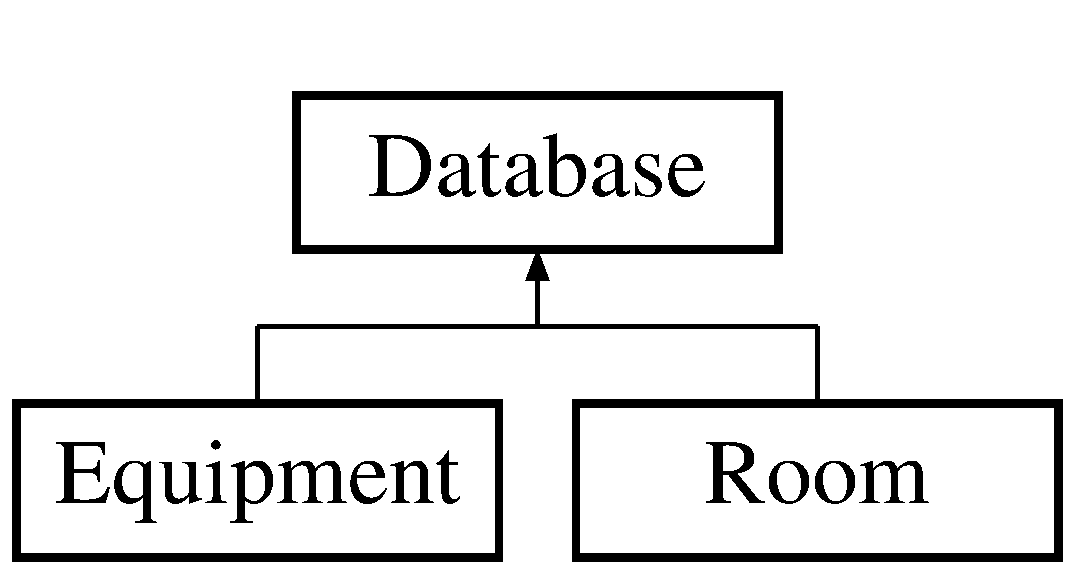
\includegraphics[height=2.000000cm]{class_database}
\end{center}
\end{figure}
\subsection*{Public Member Functions}
\begin{DoxyCompactItemize}
\item 
\mbox{\Hypertarget{class_database_af8eae4e47965e425afd92992ef6502eb}\label{class_database_af8eae4e47965e425afd92992ef6502eb}} 
virtual void {\bfseries add} ()=0
\item 
\mbox{\Hypertarget{class_database_af56afcc7b25e6e72b500a51bfe5fbba8}\label{class_database_af56afcc7b25e6e72b500a51bfe5fbba8}} 
virtual void {\bfseries remove} ()=0
\item 
\mbox{\Hypertarget{class_database_a260341c4a0f82d846f766b1718372eca}\label{class_database_a260341c4a0f82d846f766b1718372eca}} 
bool {\bfseries is\+\_\+in\+Use} ()
\item 
\mbox{\Hypertarget{class_database_a339260d3319b3e385341e8950fd52d18}\label{class_database_a339260d3319b3e385341e8950fd52d18}} 
bool {\bfseries is\+\_\+not\+Avail} ()
\end{DoxyCompactItemize}
\subsection*{Protected Attributes}
\begin{DoxyCompactItemize}
\item 
\mbox{\Hypertarget{class_database_abe3bd4bc76e3a9a78ffc9ab1cf2d313a}\label{class_database_abe3bd4bc76e3a9a78ffc9ab1cf2d313a}} 
bool {\bfseries in\+Use}
\item 
\mbox{\Hypertarget{class_database_aa603cdef357e7c119ebbcb31f3d23c81}\label{class_database_aa603cdef357e7c119ebbcb31f3d23c81}} 
bool {\bfseries not\+Avail}
\item 
\mbox{\Hypertarget{class_database_a99264fc3ee90a65147d4a2919346ff16}\label{class_database_a99264fc3ee90a65147d4a2919346ff16}} 
string {\bfseries timestamp}
\end{DoxyCompactItemize}


The documentation for this class was generated from the following files\+:\begin{DoxyCompactItemize}
\item 
C\+:/\+Users/\+Tommy B/\+Source/\+Repos/\+U\+C\+C\+S/\+Pt 3/\+Code Templates/\+Live/\+Templates/\+Templates/Database.\+h\item 
C\+:/\+Users/\+Tommy B/\+Source/\+Repos/\+U\+C\+C\+S/\+Pt 3/\+Code Templates/\+Live/\+Templates/\+Templates/Database.\+cpp\end{DoxyCompactItemize}

\hypertarget{class_database_manager}{}\section{Database\+Manager Class Reference}
\label{class_database_manager}\index{Database\+Manager@{Database\+Manager}}
\subsection*{Public Member Functions}
\begin{DoxyCompactItemize}
\item 
\mbox{\Hypertarget{class_database_manager_af2aade5b44f41d76da7a45fc340fee47}\label{class_database_manager_af2aade5b44f41d76da7a45fc340fee47}} 
void {\bfseries menu} ()
\item 
\mbox{\Hypertarget{class_database_manager_aec29b664c100048a1c02c2df4eec506b}\label{class_database_manager_aec29b664c100048a1c02c2df4eec506b}} 
\hyperlink{class_u_c_c_schedule}{U\+C\+C\+Schedule} {\bfseries get\+\_\+schedule} () const
\item 
\mbox{\Hypertarget{class_database_manager_a150d8ec849d6c6dc1a38f58274c1cf1b}\label{class_database_manager_a150d8ec849d6c6dc1a38f58274c1cf1b}} 
void {\bfseries find\+\_\+conference} ()
\item 
\mbox{\Hypertarget{class_database_manager_a485ffb37b641c6f02acd8f3444b589b1}\label{class_database_manager_a485ffb37b641c6f02acd8f3444b589b1}} 
void {\bfseries find\+\_\+session} ()
\item 
\mbox{\Hypertarget{class_database_manager_a069228cc6ef2d5aad47cdd41a96be9b9}\label{class_database_manager_a069228cc6ef2d5aad47cdd41a96be9b9}} 
void {\bfseries find\+\_\+resource} ()
\item 
\mbox{\Hypertarget{class_database_manager_a1883656160d383dd47d028244c79a67f}\label{class_database_manager_a1883656160d383dd47d028244c79a67f}} 
void {\bfseries remove\+\_\+conference} ()
\item 
\mbox{\Hypertarget{class_database_manager_ab18894c8d03100ffd9a1267634df7ce2}\label{class_database_manager_ab18894c8d03100ffd9a1267634df7ce2}} 
void {\bfseries remove\+\_\+session} ()
\item 
\mbox{\Hypertarget{class_database_manager_a5b869f71ae94cde847bdd11456cf6052}\label{class_database_manager_a5b869f71ae94cde847bdd11456cf6052}} 
void {\bfseries remove\+\_\+resource} ()
\item 
\mbox{\Hypertarget{class_database_manager_a9d5fadb956cc62b47e74452eb3422593}\label{class_database_manager_a9d5fadb956cc62b47e74452eb3422593}} 
void {\bfseries restore\+\_\+resource} ()
\end{DoxyCompactItemize}


The documentation for this class was generated from the following files\+:\begin{DoxyCompactItemize}
\item 
C\+:/\+Users/\+Tommy B/\+Source/\+Repos/\+U\+C\+C\+S/\+Pt 3/\+Code Templates/\+Live/\+Templates/\+Templates/Database\+Manager.\+h\item 
C\+:/\+Users/\+Tommy B/\+Source/\+Repos/\+U\+C\+C\+S/\+Pt 3/\+Code Templates/\+Live/\+Templates/\+Templates/Database\+Manager.\+cpp\end{DoxyCompactItemize}

\hypertarget{class_equipment}{}\section{Equipment Class Reference}
\label{class_equipment}\index{Equipment@{Equipment}}
Inheritance diagram for Equipment\+:\begin{figure}[H]
\begin{center}
\leavevmode
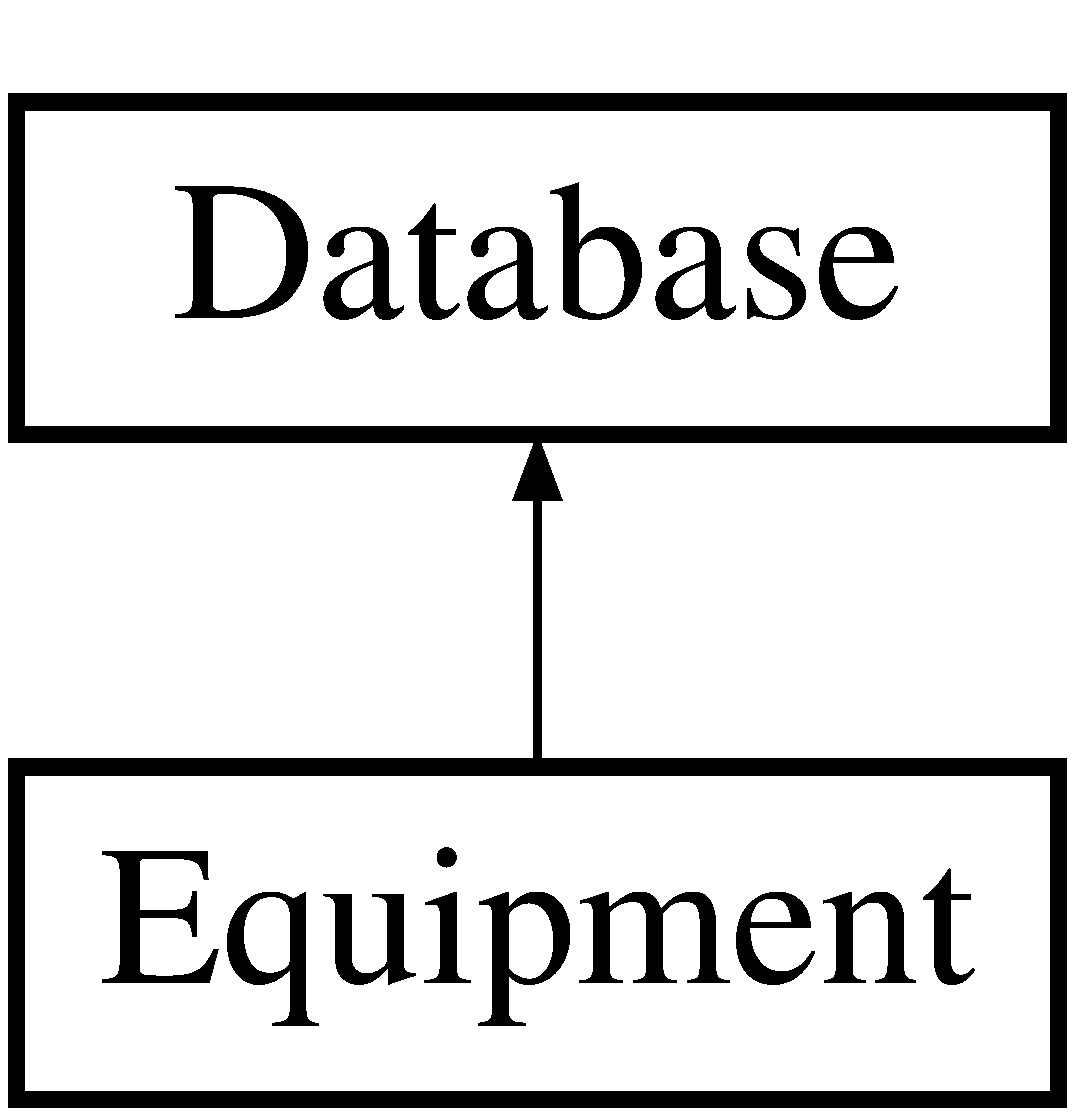
\includegraphics[height=2.000000cm]{class_equipment}
\end{center}
\end{figure}
\subsection*{Public Member Functions}
\begin{DoxyCompactItemize}
\item 
\mbox{\Hypertarget{class_equipment_a3b93df344783b00c53339a689b529e23}\label{class_equipment_a3b93df344783b00c53339a689b529e23}} 
void {\bfseries add} ()
\item 
\mbox{\Hypertarget{class_equipment_ae387f95252f51394a117d261f215ffb0}\label{class_equipment_ae387f95252f51394a117d261f215ffb0}} 
void {\bfseries remove} ()
\end{DoxyCompactItemize}
\subsection*{Additional Inherited Members}


The documentation for this class was generated from the following files\+:\begin{DoxyCompactItemize}
\item 
C\+:/\+Users/\+Tommy B/\+Source/\+Repos/\+U\+C\+C\+S/\+Pt 3/\+Code Templates/\+Live/\+Templates/\+Templates/Equipment.\+h\item 
C\+:/\+Users/\+Tommy B/\+Source/\+Repos/\+U\+C\+C\+S/\+Pt 3/\+Code Templates/\+Live/\+Templates/\+Templates/Equipment.\+cpp\end{DoxyCompactItemize}

\hypertarget{class_guest_account}{}\section{Guest\+Account Class Reference}
\label{class_guest_account}\index{Guest\+Account@{Guest\+Account}}
\subsection*{Public Member Functions}
\begin{DoxyCompactItemize}
\item 
\mbox{\Hypertarget{class_guest_account_abe433e1123fc6d762c0bca54518d199a}\label{class_guest_account_abe433e1123fc6d762c0bca54518d199a}} 
void {\bfseries menu} ()
\item 
\mbox{\Hypertarget{class_guest_account_a5c1302608d34261881d2b02a48ddafa9}\label{class_guest_account_a5c1302608d34261881d2b02a48ddafa9}} 
\hyperlink{class_u_c_c_schedule}{U\+C\+C\+Schedule} {\bfseries get\+\_\+schedule} () const
\item 
\mbox{\Hypertarget{class_guest_account_af266900055fc43ab94462f8dd3e083ac}\label{class_guest_account_af266900055fc43ab94462f8dd3e083ac}} 
void {\bfseries find\+\_\+conference} ()
\item 
\mbox{\Hypertarget{class_guest_account_affffc64177e9833403d2bebadfca3656}\label{class_guest_account_affffc64177e9833403d2bebadfca3656}} 
\hyperlink{class_conference}{Conference} {\bfseries get\+\_\+conference} () const
\item 
\mbox{\Hypertarget{class_guest_account_a1203300de0cf960e29eec88ee9098686}\label{class_guest_account_a1203300de0cf960e29eec88ee9098686}} 
void {\bfseries set\+\_\+conference\+\_\+info} ()
\item 
\mbox{\Hypertarget{class_guest_account_afb849267314653cf3d2f3e6eb0ec8930}\label{class_guest_account_afb849267314653cf3d2f3e6eb0ec8930}} 
void {\bfseries register\+\_\+guest} ()
\item 
\mbox{\Hypertarget{class_guest_account_a84e19d8ff02a1ecdb9e25b5d8b373018}\label{class_guest_account_a84e19d8ff02a1ecdb9e25b5d8b373018}} 
void {\bfseries register\+\_\+session} ()
\item 
\mbox{\Hypertarget{class_guest_account_a397df59ffa03ef48564951fbf714fe31}\label{class_guest_account_a397df59ffa03ef48564951fbf714fe31}} 
void {\bfseries modify\+\_\+sessions} ()
\item 
\mbox{\Hypertarget{class_guest_account_a34e029bd37af266012cd131a6dfa8fc5}\label{class_guest_account_a34e029bd37af266012cd131a6dfa8fc5}} 
void {\bfseries pay\+\_\+invoice} ()
\end{DoxyCompactItemize}


The documentation for this class was generated from the following files\+:\begin{DoxyCompactItemize}
\item 
C\+:/\+Users/\+Tommy B/\+Source/\+Repos/\+U\+C\+C\+S/\+Pt 3/\+Code Templates/\+Live/\+Templates/\+Templates/Guest\+Account.\+h\item 
C\+:/\+Users/\+Tommy B/\+Source/\+Repos/\+U\+C\+C\+S/\+Pt 3/\+Code Templates/\+Live/\+Templates/\+Templates/Guest\+Account.\+cpp\end{DoxyCompactItemize}

\hypertarget{class_interface}{}\section{Interface Class Reference}
\label{class_interface}\index{Interface@{Interface}}
\subsection*{Public Member Functions}
\begin{DoxyCompactItemize}
\item 
\mbox{\Hypertarget{class_interface_a4a6e24b6aa69b78733482b6941086d48}\label{class_interface_a4a6e24b6aa69b78733482b6941086d48}} 
void {\bfseries create\+\_\+account} ()
\item 
\mbox{\Hypertarget{class_interface_a334a8365e5a014f826d4c2209f9e0a39}\label{class_interface_a334a8365e5a014f826d4c2209f9e0a39}} 
void {\bfseries login\+\_\+business\+\_\+account} (string, string)
\item 
\mbox{\Hypertarget{class_interface_a8f8b4b24d3b401cad7272335dde706a4}\label{class_interface_a8f8b4b24d3b401cad7272335dde706a4}} 
void {\bfseries login\+\_\+guest\+\_\+account} (string, string)
\item 
\mbox{\Hypertarget{class_interface_ac9884793ae489dc87a9ddb5d7c0752f4}\label{class_interface_ac9884793ae489dc87a9ddb5d7c0752f4}} 
void {\bfseries login\+\_\+database\+\_\+manager} (string, string)
\end{DoxyCompactItemize}


The documentation for this class was generated from the following files\+:\begin{DoxyCompactItemize}
\item 
C\+:/\+Users/\+Tommy B/\+Source/\+Repos/\+U\+C\+C\+S/\+Pt 3/\+Code Templates/\+Live/\+Templates/\+Templates/Interface.\+h\item 
C\+:/\+Users/\+Tommy B/\+Source/\+Repos/\+U\+C\+C\+S/\+Pt 3/\+Code Templates/\+Live/\+Templates/\+Templates/Interface.\+cpp\end{DoxyCompactItemize}

\hypertarget{class_room}{}\section{Room Class Reference}
\label{class_room}\index{Room@{Room}}
Inheritance diagram for Room\+:\begin{figure}[H]
\begin{center}
\leavevmode
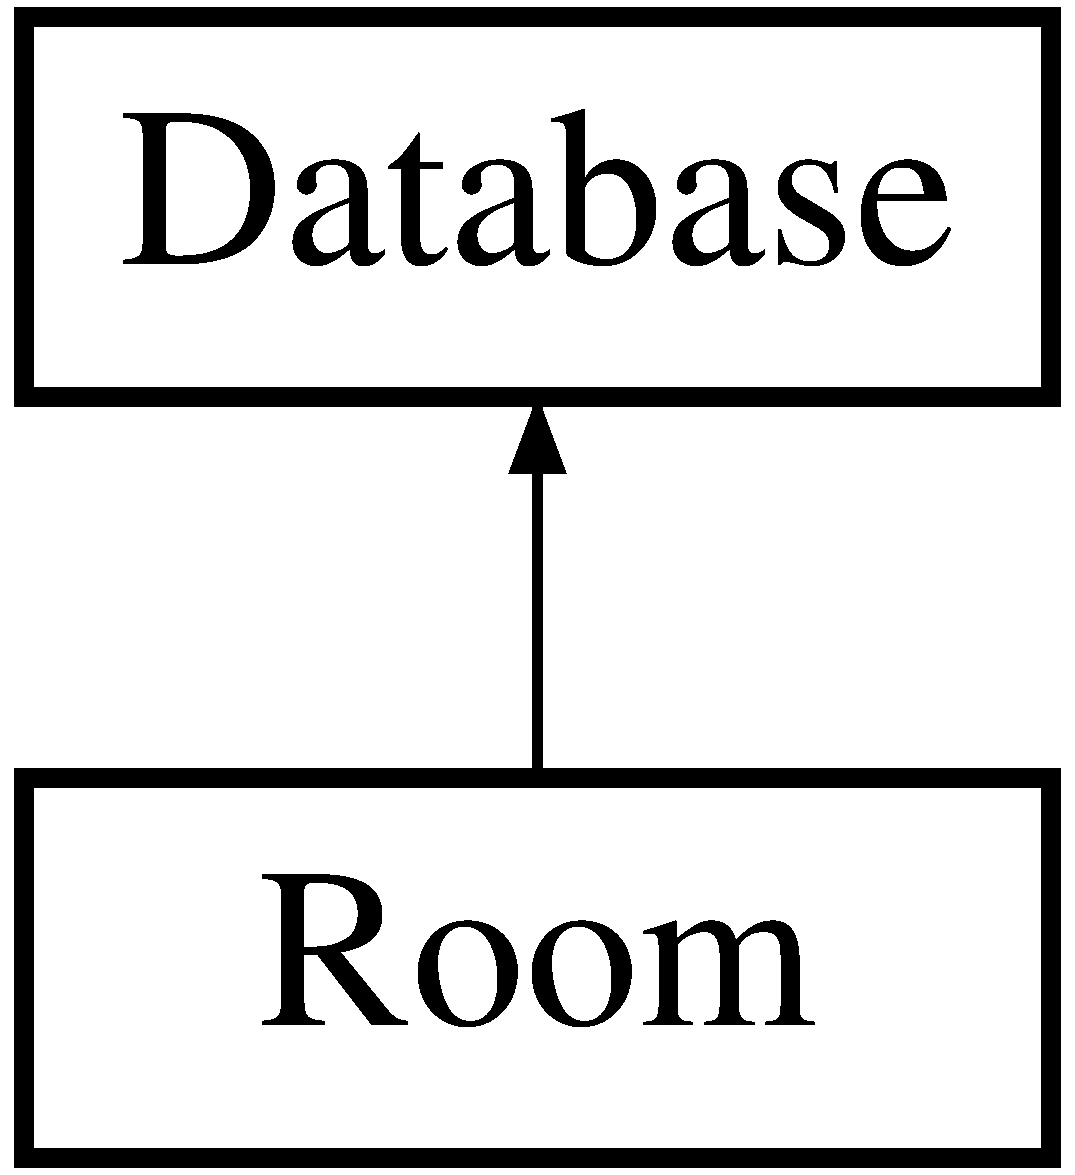
\includegraphics[height=2.000000cm]{class_room}
\end{center}
\end{figure}
\subsection*{Public Member Functions}
\begin{DoxyCompactItemize}
\item 
\mbox{\Hypertarget{class_room_af603fb655ef454d8664ade216502000d}\label{class_room_af603fb655ef454d8664ade216502000d}} 
void {\bfseries add} ()
\item 
\mbox{\Hypertarget{class_room_abc70c4d3ce84a2fd28b926bf36c8e13d}\label{class_room_abc70c4d3ce84a2fd28b926bf36c8e13d}} 
void {\bfseries remove} ()
\end{DoxyCompactItemize}
\subsection*{Additional Inherited Members}


The documentation for this class was generated from the following files\+:\begin{DoxyCompactItemize}
\item 
C\+:/\+Users/\+Tommy B/\+Source/\+Repos/\+U\+C\+C\+S/\+Pt 3/\+Code Templates/\+Live/\+Templates/\+Templates/Room.\+h\item 
C\+:/\+Users/\+Tommy B/\+Source/\+Repos/\+U\+C\+C\+S/\+Pt 3/\+Code Templates/\+Live/\+Templates/\+Templates/Room.\+cpp\end{DoxyCompactItemize}

\hypertarget{class_session}{}\section{Session Class Reference}
\label{class_session}\index{Session@{Session}}
Inheritance diagram for Session\+:\begin{figure}[H]
\begin{center}
\leavevmode
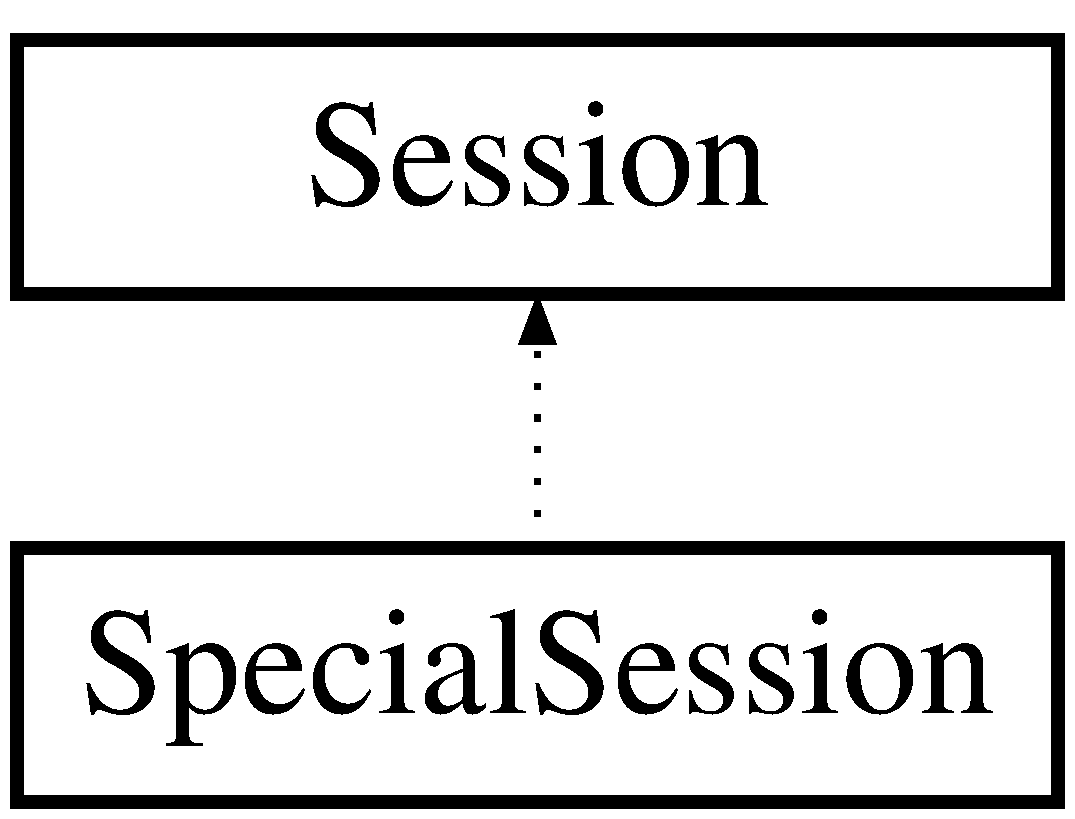
\includegraphics[height=2.000000cm]{class_session}
\end{center}
\end{figure}
\subsection*{Public Member Functions}
\begin{DoxyCompactItemize}
\item 
\mbox{\Hypertarget{class_session_a39c8482b1065e7f7ed9e356696e2293c}\label{class_session_a39c8482b1065e7f7ed9e356696e2293c}} 
void {\bfseries add\+\_\+equipment} ()
\end{DoxyCompactItemize}


The documentation for this class was generated from the following files\+:\begin{DoxyCompactItemize}
\item 
C\+:/\+Users/\+Tommy B/\+Source/\+Repos/\+U\+C\+C\+S/\+Pt 3/\+Code Templates/\+Live/\+Templates/\+Templates/Session.\+h\item 
C\+:/\+Users/\+Tommy B/\+Source/\+Repos/\+U\+C\+C\+S/\+Pt 3/\+Code Templates/\+Live/\+Templates/\+Templates/Session.\+cpp\end{DoxyCompactItemize}

\hypertarget{class_special_session}{}\section{Special\+Session Class Reference}
\label{class_special_session}\index{Special\+Session@{Special\+Session}}
Inheritance diagram for Special\+Session\+:\begin{figure}[H]
\begin{center}
\leavevmode
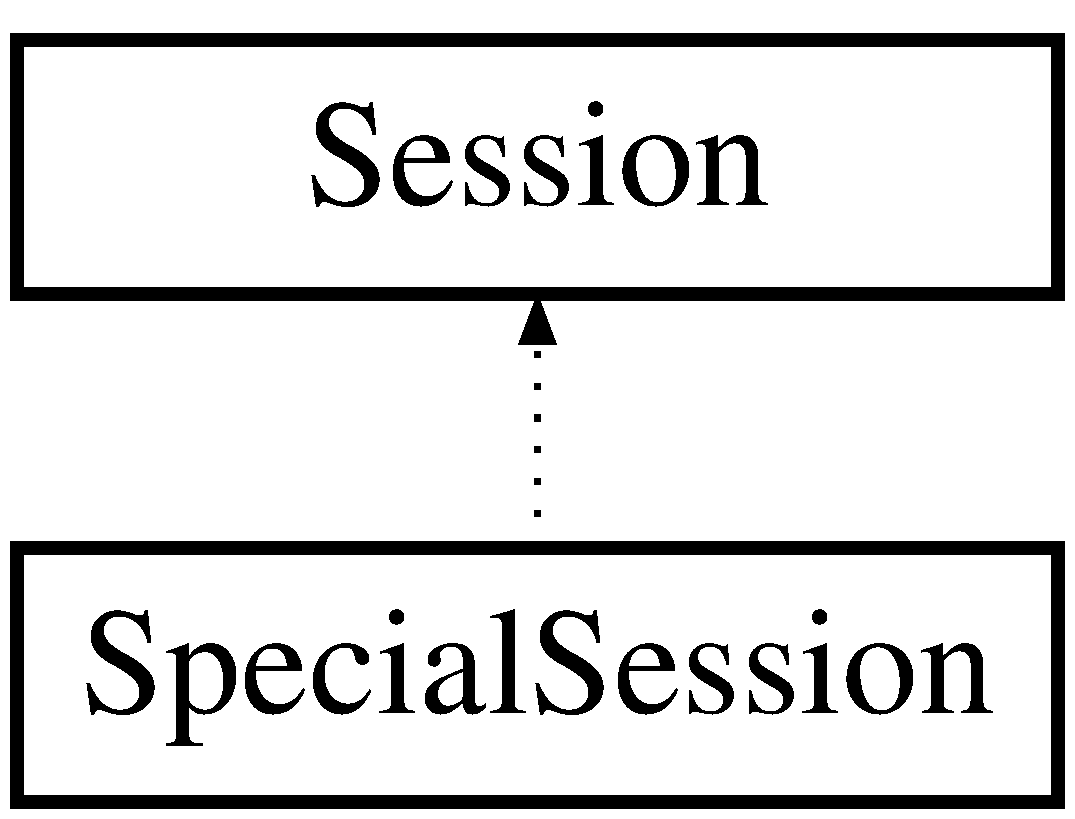
\includegraphics[height=2.000000cm]{class_special_session}
\end{center}
\end{figure}


The documentation for this class was generated from the following file\+:\begin{DoxyCompactItemize}
\item 
C\+:/\+Users/\+Tommy B/\+Source/\+Repos/\+U\+C\+C\+S/\+Pt 3/\+Code Templates/\+Live/\+Templates/\+Templates/Special\+Session.\+h\end{DoxyCompactItemize}

\hypertarget{class_u_c_c_schedule}{}\section{U\+C\+C\+Schedule Class Reference}
\label{class_u_c_c_schedule}\index{U\+C\+C\+Schedule@{U\+C\+C\+Schedule}}


The documentation for this class was generated from the following files\+:\begin{DoxyCompactItemize}
\item 
C\+:/\+Users/\+Tommy B/\+Source/\+Repos/\+U\+C\+C\+S/\+Pt 3/\+Code Templates/\+Live/\+Templates/\+Templates/U\+C\+C\+Schedule.\+h\item 
C\+:/\+Users/\+Tommy B/\+Source/\+Repos/\+U\+C\+C\+S/\+Pt 3/\+Code Templates/\+Live/\+Templates/\+Templates/U\+C\+C\+Schedule.\+cpp\end{DoxyCompactItemize}

%--- End generated contents ---

% Index
\backmatter
\newpage
\phantomsection
\clearemptydoublepage
\addcontentsline{toc}{chapter}{Index}
\printindex

\end{document}
